% $File: report.tex
% $Date: Sun Dec 16 16:04:33 2012 +0800
% $Author: wyx <ppwwyyxxc@gmail.com>

\documentclass[a4paper]{article}
\usepackage{fontspec,zhspacing,verbatim,minted, zhmath}
\usepackage{amsmath}
\usepackage[hyperfootnotes=false,colorlinks,linkcolor=blue,anchorcolor=blue,citecolor=blue]{hyperref}
\usepackage{amssymb,amsthm,fontspec,graphicx,algpseudocode}
\usepackage[sorting=none]{biblatex}
\usepackage{subfigure}
\usepackage{textcomp,enumerate}
\usepackage{indentfirst}
\usepackage{float,chngpage}
\usepackage{titlesec}
\usepackage{fancyhdr}
\usepackage{extarrows}
\usepackage{titlesec}
\usepackage{caption}\captionsetup{hypcap=true}
\usepackage{indentfirst}
\newfontfamily\zhfont[BoldFont=SimHei,ItalicFont=KaiTi_GB2312]{SimSun}
\zhspacing


\changetext{}{2.2cm}{-1.1cm}{-1.1cm}{}
\pagestyle{fancy}
\setlength{\headheight}{15.2pt}
\lhead[]{}\rhead[]{}
%\chead[\em 探究人耳对语言的辨识]{\em 探究人耳对语言的辨识}
\fancyhead[C]{\emph{Probability Features of Random Permutations}}

%\renewcommand{\abstractname}{摘要}
%\renewcommand{\contentsname}{目录}
%\renewcommand{\figurename}{图}
%\defbibheading{bibliography}{\section{参考文献}}

\newcommand{\figref}[1]{\hyperref[fig:#1]{Figure \ref*{fig:#1}}}
\newcommand{\eqnref}[1]{\hyperref[eqn:#1]{(\ref*{eqn:#1})}}
\newcommand{\lemref}[1]{\hyperref[lemma:#1]{Lemma \ref*{lemma:#1}}}
\newcommand{\secref}[1]{\hyperref[sec:#1]{\ref*{sec:#1}节}}
\DeclareMathOperator{\LM}{\tiny{LM}}
\DeclareMathOperator{\LT}{\tiny{LT}}
\DeclareMathOperator{\rank}{\tiny{rank}}
\DeclareMathOperator{\sgn}{sgn}
\DeclareMathOperator{\Cov}{Cov}

\let\Oldsum\sum
\renewcommand{\sum}{\displaystyle\Oldsum}
\let\Oldprod\prod
\renewcommand{\prod}{\displaystyle\Oldprod}
\let\Oldcap\bigcap
\renewcommand{\bigcap}{\displaystyle\Oldcap}
\let\Oldcup\bigcup
\renewcommand{\bigcup}{\displaystyle\Oldcup}
\let\Oldint\int
\renewcommand{\int}{\displaystyle\Oldint}
\let\Oldiint\iint
\renewcommand{\iint}{\displaystyle\Oldiint}

% $File: mint-defs.tex
% $Date: Sat Feb 16 22:59:11 2013 +0800
% $Author: wyx <ppwwyyxxc@gmail.com>

\usepackage{xparse}


% \inputmintedConfigured[additional minted options]{lang}{file path}{
\newcommand{\inputmintedConfigured}[3][]{\inputminted[fontsize=\footnotesize,
	label=#3,linenos,frame=lines,framesep=0.8em,tabsize=4,#1]{#2}{#3}}

% \phpsrc[additional minted options]{file path}: show highlighted php source
\newcommand{\phpsrc}[2][]{\inputmintedConfigured[#1]{php}{#2}}
% \phpsrcpart[additional minted options]{file path}{first line}{last line}: show part of highlighted php source
\newcommand{\phpsrcpart}[4][]{\phpsrc[firstline=#3,firstnumber=#3,lastline=#4,#1]{#2}}
% \phpsrceg{example id}
\newcommand{\phpeg}[1]{\inputminted[startinline,
	firstline=2,lastline=2]{php}{res/php-src-eg/#1.php}}

\newcommand{\txtsrc}[2][]{\inputmintedConfigured[#1]{text}{#2}}
\newcommand{\txtsrcpart}[4][]{\txtsrc[firstline=#3,firstnumber=#3,lastline=#4,#1]{#2}}

\newcommand{\pysrc}[2][]{\inputmintedConfigured[#1]{py}{#2}}
\newcommand{\pysrcpart}[4][]{\pysrc[firstline=#3,firstnumber=#3,lastline=#4,#1]{#2}}

\newcommand{\confsrc}[2][]{\inputmintedConfigured[#1]{squidconf}{#2}}
\newcommand{\confsrcpart}[4][]{\confsrc[firstline=#3,firstnumber=#3,lastline=#4,#1]{#2}}

\newcommand{\cppsrc}[2][]{\inputmintedConfigured[#1]{cpp}{#2}}
\newcommand{\cppsrcpart}[4][]{\cppsrc[firstline=#3,firstnumber=#3,lastline=#4,#1]{#2}}

\renewcommand{\P}[1]{\text{P}\left(#1\right)}
\renewcommand{\Pr}[1]{\text{Pr}\left\{#1\right\}}
\newcommand{\Px}[2]{\text{P}_{#1}\left(#2\right)}
\newcommand{\E}[1]{\text{E}\left[#1\right]}
\newcommand{\Ex}[1]{\text{E}#1}
\newcommand{\Var}[1]{\text{Var}\left[#1\right]}
%\newcommand{\Cov}[2]{\text{Cov}\left[#1,#2\right]}
%\newcommand{\Cov}[1]{\text{Cov}\left[#1 \right]}
\renewcommand{\T}[1]{\Theta\left(#1\right)}
\newcommand{\real}{\mathbb{R}}
\newcommand{\card}[1]{\left\|#1\right\|}
\newtheorem{lemma}{Lemma}

\NewDocumentCommand\Cov{mg}{
    \text{Cov}\left[ #1 \IfNoValueTF{#2}{}{,#2}\right]
 }

\newcommand{\qed}{\hfill \ensuremath{\Box}}



\title{Probability Features of Random Permutations}
\author{\\(ppwwyyxxc@gmail.com)}

\begin{document}
\maketitle
\begin{abstract}
  In this paper, we will

\end{abstract}
\tableofcontents
\newpage
% $File: notation.tex
% $Date: Sun Dec 23 01:04:29 2012 +0800
% $Author: jiakai <jia.kai66@gmail.com>

\section*{Notations}
Throughout this paper, we would use the following notations:
\begin{itemize}
	\item $\Pr{S}$ is the probability of $S$ ($S$ is usually a set or a
		proposition).
	%\item $\Px{X}{x}$ is the probability distribution function for random
		%variable $X$, and if $X$ is discrete we have $\Px{X}{x} = \Pr{X = x}$.
		%We would write $\P{x}$ instead of $\Px{X}{x}$ if there is no ambiguity.
	\item $\E{X}$ is the expectation of random variable $X$, which is defined
		as the following for a discrete random variable:
		\begin{equation*}
			\E{X} = \sum_k k\P{k}
		\end{equation*}
	\item $\Var{X}$ is the variance of random variable $X$, defined as
		\begin{equation*}
			\Var{X} = \E{(X-\E{X})^2}
		\end{equation*}
	\item $\Cov[X,Y]$ is the covariance of random variables $X, Y$, defined as
		\begin{equation*}
			\Cov[X,Y] = \E{XY}-\E{X}\E{Y}
		\end{equation*}
	%\item $\T{f(n)}$ and $\O{f(n)}$ are used to describe the asymptotic behavior
		%of functions, defined as:
		%\begin{quote}
			%$f(n) = \O{g(n)}$ iff $\exists N_0, c \in \real$ such that
			%\begin{equation*}
				%\forall n > N_0, |f(n)| < c|g(n)|
			%\end{equation*}
			%$f(n) = \T{g(n)}$ iff $f(n) = \O{g(n)}$ and $g(n) = \O{f(n)}$
		%\end{quote}
\end{itemize}

% vim: filetype=tex foldmethod=marker foldmarker=f{{{,f}}}


% File: fixed_points.tex
% Date: Sun Dec 16 21:27:57 2012 +0800
% Author: Yuxin Wu <ppwwyyxxc@gmail.com>
\section{Fixed Points}
\subsection{Introduction}
Let $ \pi= (\pi(1), \pi(2),\cdots ,\pi(n))$ be a permutation of $ (1,2,\cdots ,n)$.
The \emph{\textbf{Fixed Points}} of the permutation $ \pi$ ,
denoted as $ \mathcal{F}(\pi)$, is defined as followed:
\[ \mathcal{F}(\pi) = \{ k \in [1,n]\cap \mathbb{N} \mid \pi(k) = k \}\]

Let $ \Pi_n$ be the set of all possible permutations of $ (1,2,\cdots ,n)$.
The \emph{\textbf{Rencontres Numbers}} $ D_{n,k}$ is defined as followed:
\[ D_{n,k} = \card{ \{ \pi \in \Pi_n \mid \card{\mathcal{F}(\pi)} = k \}}, k = 0,1,\cdots n\]
where $ \card{A}$ is the cardinality of a set $ A$.

In particular, when $ k = 0$, we denote $ D_{n,0}$ as $  D_{n} $ for short.

Let $ \pi $ be a random permutation of $ (1,2,\cdots ,n),$ where
every possible permutation have the same possibility $ \dfrac{1}{n!}$.
The Random Variable $ S = \card {\mathcal{F}(\pi)} $ is what we will focus on.

\subsection{Calculation of $ D_{n,k}$}
\label{sec:f-calc}
We are about to see three totally different approaches of the calculation of $ D_{n}$.

Then we can easily caculate $ D_{n,k}$ by
\[ D_{n,k} = {n\choose{k}}D_{n-k}\].

\begin{enumerate}
    \item using the Inclusion-Exclusion Principle

      Define $ A_j$ as:
      \[ A_j =  \{ \pi \in \Pi | j \in \mathcal{F}(\pi)\}, j = 1,2,\cdots ,n\]

      Then it is obvious to see that, for any $ t = 1,2,\cdots ,n$, we have
      \[ \card{\bigcap_{i=1}^{t}A_{r_i}} = (n-t)!\]
      where $ r_i$ is any permutation of $ (1,2,\cdots ,n).$

      Therefore, $ D_n$ can be calculated by the Inclusion-Exclusion Principle:
       \begin{align*}
       D_n = & n! - \sum_{i=1}^n\card{A_i} + \sum_{1\le i< j\le n}{\card{A_i\cap A_j}}-\cdots +
      (-1)^n\card{\bigcap_{i=1}^n{A_i}}\\
      =& n! - {n\choose{1}}(n-1)! + {n\choose{2}}(n-2)!-\cdots +(-1)^n{n\choose{n}}(n-n)!\\
      =& n!\sum_{i=0}^n{\dfrac{(-1)^i}{i!}}
      \end{align*}

      \item using recurrence relation

     For any permutation $\pi$ of $ (1,2,\cdots n),$ such that $ \card{\mathcal{F}(\pi) = 0}$,
     it is obvious that $ \pi(1)$ has $ n-1$ possible values.
     Now consider the value of $ \pi(\pi(1)):$

     If $ \pi(\pi(1)) = 1, $ then $\pi'= (\pi(2),\cdots ,\pi(\pi(1)-1), \pi(\pi(1)+1), \cdots ,\pi(n))$
     is a permutation of
     $ (2,\cdots ,\pi(1)-1, \pi(1)+1, \cdots ,n)$, such that $\card{\mathcal{F}(\pi')} = 0$.
     It is easy to show that this correspondence from the given $ \pi$ to $ \pi'$is bijective.

     If $ \pi(\pi(1)) \neq 1$, assume $ \pi(j) = 1$, then $ \pi' =(\pi(2), \cdots ,\pi(j-1), \pi(1), \pi(j+1), \cdots ,\pi(n))$
     is a permutation of $ (2,\cdots ,n),$ such that $\card{\mathcal{F}(\pi')}=0$.
     It is easy to show that this correspondence from the given $\pi$ to $ \pi'$ is also bijective.

     Therefore, we have the recurrence relation
\begin{align}
& D_n = (n-1)(D_{n-1}+D_{n-2}) \nonumber\\
\Leftrightarrow & D_n - nD_{n-1} = - [D_{n-1}- (n-1)D_n-2] \label{eqn:recurrence}\\
&D_2 = 1, D_1 = 0 \nonumber
\end{align}

Continue applying \eqnref{recurrence}, we obtain
\begin{align*}
 &D_n - nD_{n-1} = -[D_{n-1}-(n-1)D_{n-2}]= \cdots  =(-1)^{n-2}(D_2 - 2D_1) = (-1)^n \\
 \Rightarrow & \dfrac{D_n}{n!} - \dfrac{D_{n-1}}{(n-1)!} = \dfrac{(-1)^n}{n!} \\
 \Rightarrow &D_n = n! \sum_{i=0}^n{\dfrac{(-1)^i}{i!}}
\end{align*}

\item using the Inversion Formula
\begin{lemma}
  \textbf{(Inversion Formula)}
  \label{lemma:inversion}
  Given two arrays $ \{ a_n\},\{ b_n\} $. If the formula
  \[  b_n = \sum_{k=0}^n(-1)^k{n\choose{k}}a_k\]
  holds for any $ n = 1,2,\cdots $, then
  \[ a_n = \sum_{k=0}^n(-1)^k{n\choose{k}}b_k, n = 1,2,\cdots \]
\end{lemma}
\begin{proof}
Note that in series $ \sum_{k=0}^n(-1)^k{n\choose{k}}(1+x)^k,$
the coefficient of the term $ x^p$ is given by $
\sum_{k=p}^n(-1)^k{n\choose{k}}{k\choose{p}}.$

On the other hand, by Binomial Theorem,
\[ \sum_{k=0}^n(-1)^k{n\choose{k}}(1+x)^k = [1-(1+x)]^n = (-1)^nx^n, \]
therefore the coefficient of the term $ x^p$ is $(-1)^n\delta_{pn} $, where $ \delta_{ij}$ is the
\emph{Kronecker delta function}:
\[ \delta_{ij} = \begin{cases}
  1, i = j \\ 0, i \ne j \end{cases} \]
  Thus,
  \[ \sum_{k=p}^n(-1)^k{n\choose{k}}{k\choose{p}} = (-1)^n\delta_{pn}\]

  It follows that
\begin{align*}
    \sum_{k=0}^n(-1)^k{n\choose{k}}b_k &=
    \sum_{k=0}^n(-1)^k{n\choose{k}}\left[\sum_{p=0}^k(-1)^i{k\choose{i}}a_i\right] \\
    &=\sum_{p=0}^n(-1)^p\left[\sum_{k=p}^n(-1)^k{n\choose{k}}{k\choose{p}}a_p\right] \\
   &=\sum_{p=0}^n(-1)^p(-1)^n\delta_{pn}a_p = a_n
\end{align*} \end{proof}

By definition, $ \sum_{k=0}^nD_{n,k} =\card{\Pi_n}= n!$,
which is equivalent to
 \begin{equation}
 n! = \sum_{k=0}^n{n\choose{k}}D_k =
  \sum_{k=0}^n\left[ (-1)^k{n\choose{k}}\right]\left[(-1)^kD_k\right]
  \label{eqn:fact}
  \end{equation}

According to \lemref{inversion}, we immediately obtain:
\begin{align*}
&(-1)^nD_n = \sum_{k=0}^n(-1)^k{n\choose{k}}k! \\
\Rightarrow & D_n = \sum_{k=0}^n(-1)^{n-k}\dfrac{n!}{(n-k)!} = n!\sum_{k=0}^n\dfrac{(-1)^k}{k!}
\end{align*}
\end{enumerate}

\subsection{On the Random Variable $ S$}
\label{f-random}
By definition, the probability mass function of $ S$ is given by
  \begin{equation}
  \Pr{S=k} = \dfrac{D_{n,k}}{n!}=\dfrac{{n\choose{k}}D_{n-k}}{n!}, k = 0,1,\cdots ,n
  \label{eqn:f-pr}
  \end{equation}

Then the expectation of $ S$ can be calculated as followed:
\[ \E{S} = \sum_{k=0}^n\dfrac{k{n\choose{k}}D_{n-k}}{n!} = \sum_{k=0}^n\dfrac{n{n-1\choose{n-k}}D_{n-k}}{n!} =
  \sum_{k=0}^n\dfrac{{n-1\choose{n-k}}D_{n-k}}{(n-1)!} = 1 \]
Recall that $ \sum_{k=0}^n{n-1 \choose{n-k}}D_{n-k}=(n-1)!$ according to \eqnref{fact}.

By similiar approach, the variance can also be derived:
\[ \E{S(S-1)} = \sum_{k=0}^n\dfrac{k(k-1){n\choose k}D_{n-k}}{n!}\sum_{k=0}^n\dfrac{n(n-1){n-2 \choose{n-k}}D_{n-k}}{n!} = 1\]
\[ \Var{S} = \E{S(S-1)} + \E{S}-\E{S}^2 = 1\]
\\

Another way of calculating expectation and variance is by treating $ S$ as a sum of $ n $ identical
random variable $ X_i$, where $ X_i$ is defined by:
\[ X_i = \begin{cases}1, \pi(i)=i\\0,\pi(i)\neq i\end{cases}\]
Obviously $ S = \sum_{i=1}^nX_i$ and $ X_i\sim b(1,\dfrac{1}{n})$, where $ b(n,p)$ denotes the
binomial distribution with sample size $ n$ and success probability $ p$.

It can be easily shown that for $ i\neq j, \Pr{X_iX_j=1}=\dfrac{(n-2)!}{n!}=\dfrac{1}{n(n-1)} $, therefore $X_iX_j \sim b(1, \dfrac{1}{n(n-1)})$.

Then we can obtain:
\[ \E{S} = \sum_{i=1}^n\E{X_i} = 1\]
\[ \Cov[X_i,X_j]=\E{X_iX_j}-\E{X_i}\E{X_j}=\dfrac{1}{n^2(n-1)}\]
\[ \Var{S} = \sum_{i=1}^n\Var{X_i}+\sum_{i\neq j}\Cov[X_i,X_j] = 1\]

\subsection{Connections to Gamma Function}
Continue working on \eqnref{f-pr}, we can obtain:
\[ \Pr{S=k} = \dfrac{{n\choose{k}}}{n!}(n-k)!\sum_{i=0}^{n-k}{\dfrac{(-1)^i}{i!}} = \dfrac{1}{k!}\sum_{i=0}^{n-k}\dfrac{(-1)^i}{i!}\]

Introducing the \emph{incomplete gamma function} defined as:
\[ \Gamma(s,x) = \int_{x}^{\infty}t^{s-1}e^{-t}\mathrm{d}t\]
By integration by parts, a recurrence relation can be found:
\[ \Gamma(s,x) = (s-1)\Gamma(s-1,x) + x^{s-1}e^{-x}\]
Thus,
\[\forall n\in \mathbb{N}, \Gamma(n,x) = (n-1)! e^{-x}\sum_{i=0}^{n-1}\dfrac{x^i}{i!}\]
We can then rewrite the previous formula in a more elegant way:
\[ D_n = \dfrac{\Gamma(n+1, -1)}{e}\]
\[ \Pr{S=k}=\dfrac{{n\choose{k}}\Gamma(n-k+1,-1)}{en!} =\dfrac{\Gamma(n-k+1,-1)}{ek!(n-k)!}\]
\\

Another way of rewriting $ D_n$ is:
\[ D_n = \E{(X-1)^n}\]
where $ X$ is a random variable such that $ X\sim Exp(1),$
here  $Exp(\lambda) $ denotes exponential distribution.

To prove this, it is sufficient to show that
\[ \E{X^k} = \int_{\mathbb{R}^+}x^ke^{-x} = \Gamma(k+1) = k!\]
where $ \Gamma(x)$ is the complete gamma function.

Thus,
\[ \E{(X-1)^n} = \sum_{k=0}^n{n\choose{k}}\E{X^{n-k}}(-1)^k = \sum_{k=0}^n{n\choose k}(-1)^k(n-k)! = D_n\]

\subsection{Approximation}
Note that $ e^{-1} = \sum_{i=0}^{\infty}\dfrac{(-1)^i}{i!}$,
which indicates that $D_n \approx e^{-1}n!, \Pr{S=k}\approx \dfrac{e^{-1}}{k!}$.

Therefore when $ n$ is large enough,
$ S$ approximately obeys Poisson distribution with the parameter $ 1$.

Actually, even when $ n$ is small,
there is very little difference between $ \Pr{S=k}$ and $ \dfrac{1}{ek!}$,
as shown in \figref{diff}.

\begin{figure}[H]
  \centering
  \subfigure[$n$=3]{
    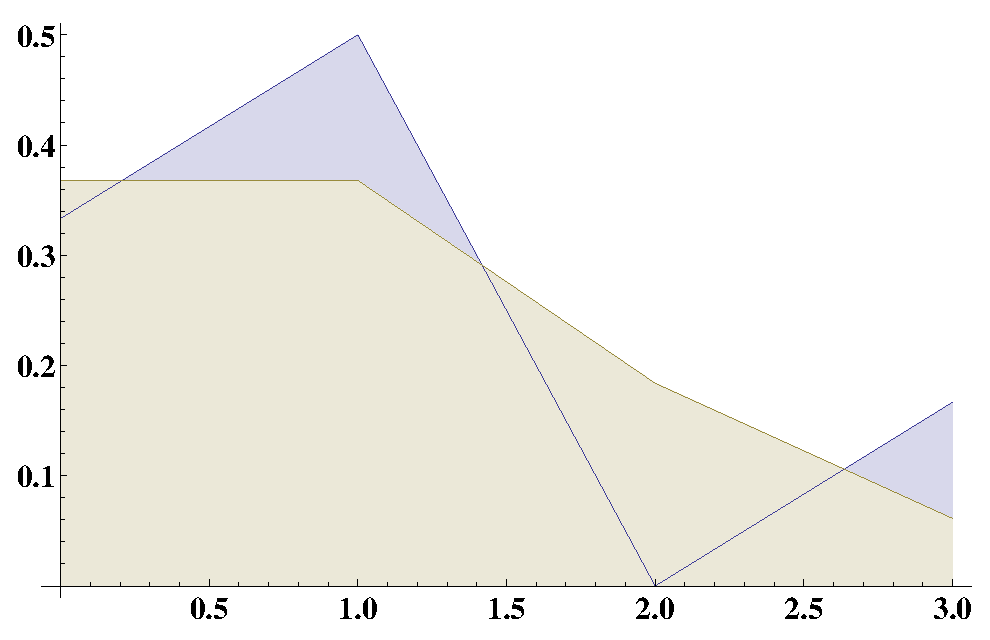
\includegraphics[scale=0.4]{pics/n3.eps}
  }
  \subfigure[$ n$=4]{
    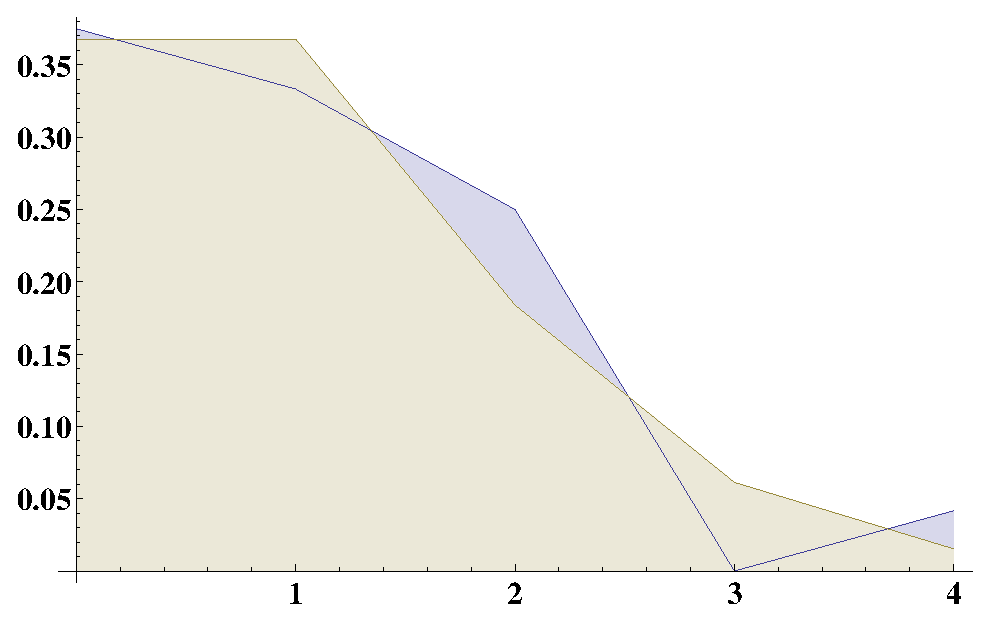
\includegraphics[scale=0.4]{pics/n4.eps}
  }
  \subfigure[$n$=5]{
  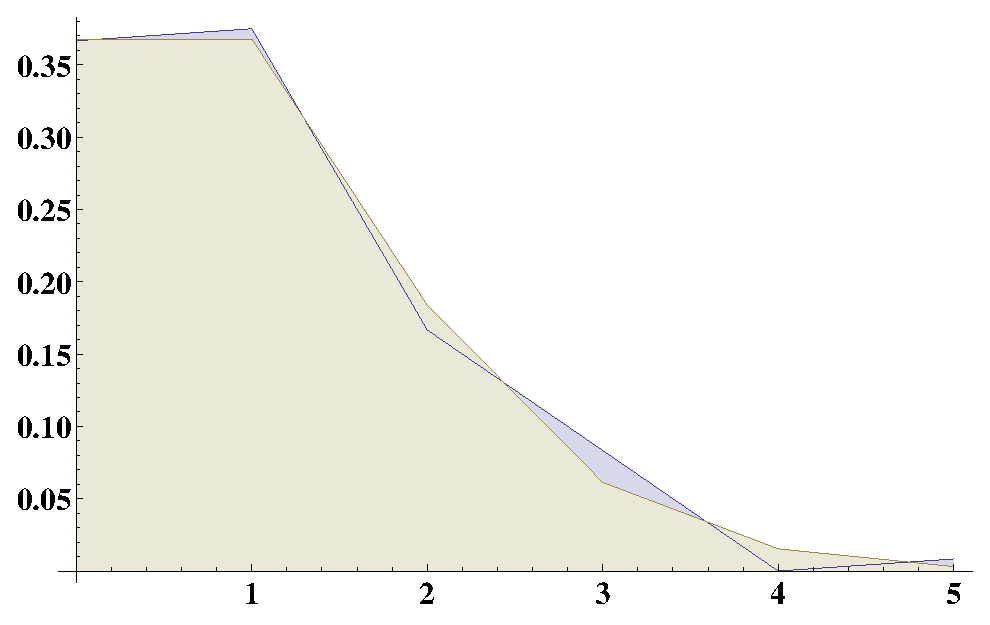
\includegraphics[scale=0.4]{pics/n5.eps}
  }
  \subfigure[$ n$=6]{
  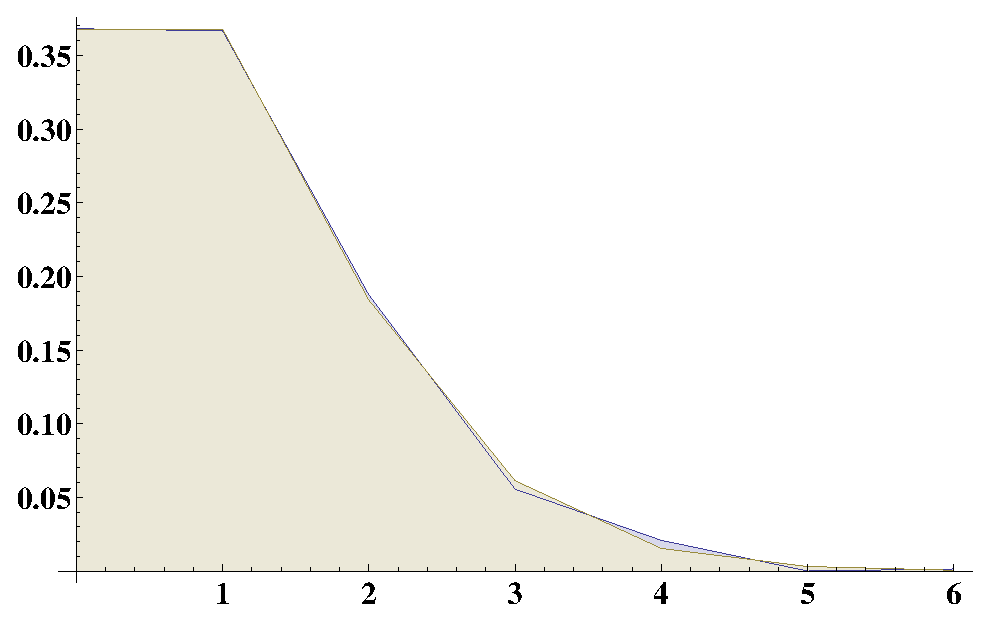
\includegraphics[scale=0.4]{pics/n6.eps}
  }
  \caption{Values of $ \Pr{S=k}$ and $ \dfrac{1}{ek!}$\label{fig:diff}}
\end{figure}

We can then conclude that Poisson distribution is a very good approximation to $ S$.
\\

Inspired by the previous discusson, we now consider the difference between $ D_n $ and $ e^{-1}n!$.

It is obvious that
\begin{align*}
|n! e^{-1} - D_n| & \le \dfrac{1}{(n+1)}+\dfrac{1}{(n+1)(n+2)}+ \dfrac{1}{(n+1)(n+2)(n+3)}+\cdots \\
&< \dfrac{1}{(n+1)} + \dfrac{1}{(n+1)^2 }+ \cdots  \\
& =\dfrac{1}{n}\\
& \le \dfrac{1}{2} ( n \ge 2)
\end{align*}
And for $ n=1,$ we still have $ |n!e^{-1}-D_n| < \dfrac{1}{2}.$

But knowing that $ D_n$ is an integer, we immediately get
\[  D_n = [ n!e^{-1}],\] where $ [x]$ denote the nearest integer of $ x$, and
\[ \Pr{S=k} = \dfrac{{n\choose{k}}[(n-k)!e^{-1}]}{n!}= \dfrac{[(n-k)!e^{-1}]}{k!(n-k)!}\]
We can then obtain a profound result:
\[ \lim\limits_{n\to\infty}\Pr{S=0} = \dfrac{1}{e}\]



\end{document}

